% !TEX TS-program = pdflatex
% !TEX encoding = UTF-8 Unicode

\documentclass[a4paper, titlepage=false, parskip=full-, 10pt]{scrartcl}

\usepackage[utf8]{inputenc}
\usepackage[T1]{fontenc}
\usepackage[english, ngerman]{babel}
\usepackage{babelbib}
\usepackage{hyperref}
\usepackage{listings}
\usepackage{framed}
\usepackage{color}
\usepackage{graphicx}
\usepackage[normalem]{ulem}
\usepackage{cancel}
\usepackage{amsmath}
\usepackage{amssymb}
\usepackage{amsthm}
\usepackage{algorithm}
\usepackage{algorithmic}
\usepackage{geometry}
\usepackage{subfigure}
\geometry{a4paper, top=20mm, left=35mm, right=25mm, bottom=40mm}

\newcounter{tasknbr}
\setcounter{tasknbr}{1}
\newenvironment{task}[1]{{\bf Aufgabe \arabic {tasknbr}\stepcounter{tasknbr}} (#1):\begin{enumerate}}{\end{enumerate}}
\newcommand{\subtask}[1]{\item[#1)]}

% Listings -----------------------------------------------------------------------------
\definecolor{red}{rgb}{.8,.1,.2}
\definecolor{blue}{rgb}{.2,.3,.7}
\definecolor{lightyellow}{rgb}{1.,1.,.97}
\definecolor{gray}{rgb}{.7,.7,.7}
\definecolor{darkgreen}{rgb}{0,.5,.1}
\definecolor{darkyellow}{rgb}{1.,.7,.3}
\lstloadlanguages{C++,[Objective]C,Java}
\lstset{
escapeinside={§§}{§§},
basicstyle=\ttfamily\footnotesize\mdseries,
columns=fullflexible,
keywordstyle=\bfseries\color{blue},
commentstyle=\color{darkgreen},      
stringstyle=\color{red},
numbers=left,
numberstyle=\ttfamily\scriptsize\color{gray},
breaklines=true,
showstringspaces=false,
tabsize=4,
captionpos=b,
float=htb,
frame=tb,
frameshape={RYR}{y}{y}{RYR},
rulecolor=\color{black},
xleftmargin=15pt,
xrightmargin=4pt,
aboveskip=\bigskipamount,
belowskip=\bigskipamount,
backgroundcolor=\color{lightyellow},
extendedchars=true,
belowcaptionskip=15pt}

%% Enter current values here: %%
\newcommand{\lecture}{Robotik WS15/16}
\newcommand{\tutor}{}
\newcommand{\assignmentnbr}{3}
\newcommand{\students}{Julius Auer}
%%-------------------------------------%%

\begin{document}  
{\small \textsl{\lecture \hfill \tutor}}
\hrule
\begin{center}
\textbf{Übungsblatt \assignmentnbr}\\
[\bigskipamount]
{\small \students}
\end{center}
\hrule

\begin{task}{Koordinaten-Transformation}
\subtask{a}
Annahme: die Winkel sollen fest sein und ''irgendwie'' aus der Skizze abgelesen werden.

Im vorliegenden Fall sieht es nämlich auch so aus, als könne man sich die mühselige Rotation um Euler-Winkel sparen und die Rotation - die hier wohl nur einem Tauschen der Achsen-Labels und Richtungen entspricht - aus der Skizze ablesen zu:
$$^A_BR=\begin{pmatrix}0&-1&0\\-1&0&0\\0&0&-1\end{pmatrix}$$

Nun ist im Weiteren die Notation der Aufgabe etwas irreführend: man sollte meinen, $^A_BT$ überführt {\bf von} dem System $A$ {\bf nach} $B$ - im verbalen Teil ist jedoch der umgekehrte Fall beschrieben. Nunja, für die Rotation spielt das ohnehin keine Rolle, da hier
$$^A_BR=^A_BR^T=^B_AR$$
für die Translation jedoch sehr wohl. Ich nehme mal den einfacheren Fall an, dass ein in $B$ gegebener Vektor in $A$ beschrieben werden soll (was auch besser zum Rest der Aufgabe passt ...). Dann gilt:
$$^A_BT=\begin{pmatrix}&^A_BR&&^AP_{Borg}\\0&0&0&1\end{pmatrix}$$

\subtask{b}
\begin{align*}
v_A&=^A_BT\cdot v_B\\
&=\begin{pmatrix}0&-1&0&-3\\-1&0&0&-2\\0&0&-1&-2\\0&0&0&1\end{pmatrix}\cdot\begin{pmatrix}1\\-2\\3\\1\end{pmatrix}=\begin{pmatrix}2-3\\-1-2\\-3-2\\1\end{pmatrix}\hat{=}\begin{pmatrix}-1\\-3\\-5\end{pmatrix}
\end{align*}
\end{task}

\begin{task}{Kommunikation zwischen ROS-Nodes}
\subtask{a}
Einzig erwähnenswertes: implementiert man mit Python dauert es recht lange bis die Callback-Threads starten - der Aufruf kommt aber sofort zurück, weshalb ein \emph{sleep} vonnöten war. Ansonsten straight-forward. Abbildung \ref{fig:2-1} zeigt das Resultat, Code liegt im Sakai.

\begin{figure}[!htpb]
\centering
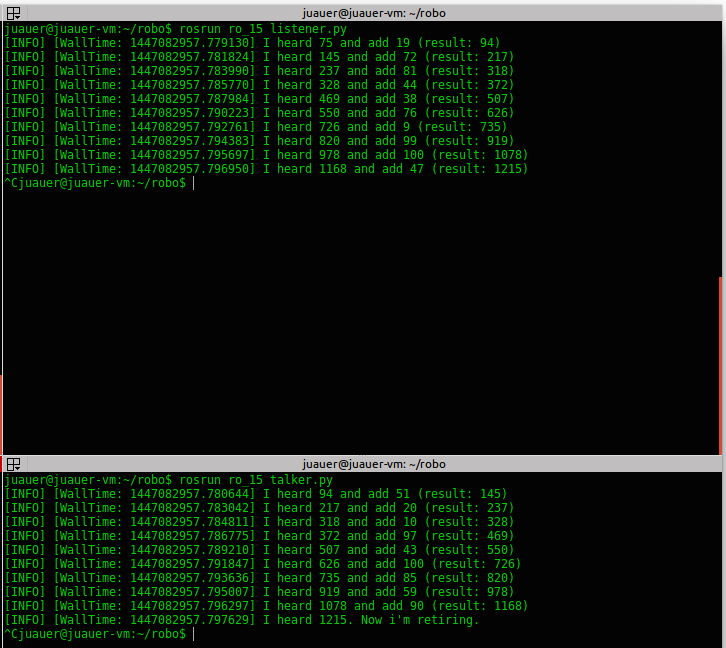
\includegraphics[width=0.9\linewidth]{capture_2-1}
\caption{Talker und Listener}
\label{fig:2-1}
\end{figure}

\subtask{b}
Der Code um Joint-Positionen zu setzen war ja mehr oder weniger vorgegeben. Ich inkrementiere einen Winkel $th$ um $0.1$ pro Schleifendurchlauf und setze den unteren Joint auf $sin(th)$ und den oberen auf $cos(th)$.

Um den Abstand zum Ursprung zu plotten bin ich dem Vorschlag gefolgt ein ''virtuelles'' Gelenk (Box mit Ausdehnung 0 0 0) \emph{virtual\_link} dem Modell hinzuzufügen. Die Transformation von \emph{/virtual\_link} nach \emph{/base\_link} liefert dann den gesuchten Vektor, dessen Länge geplottet werden soll.

Hierfür habe ich einen zusätzlichen Publisher eingerichtet, der die euklidsche Länge des Vektors \emph{link\_virt} published. Dieser Wert kann dann komfortabel mit rqt\_plot geplottet (Abbildung \ref{fig:2-2}) oder auf der Konsole mit \emph{rostopic echo /link\_virt} observiert werden.

\begin{figure}[!htpb]
\centering
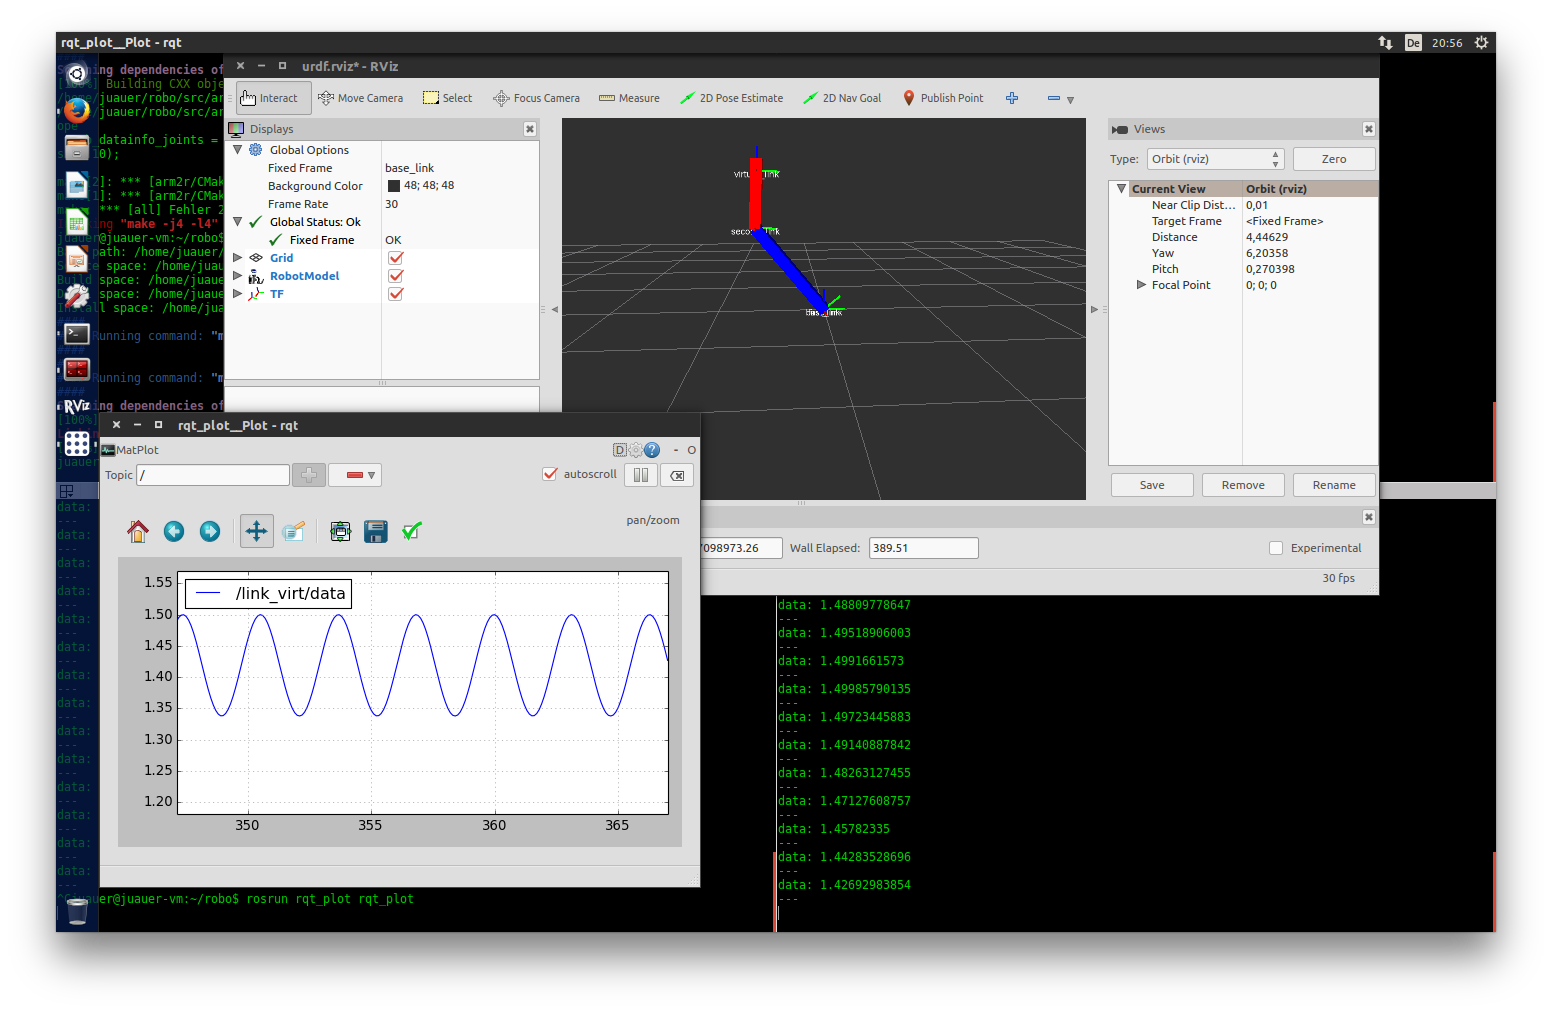
\includegraphics[width=0.9\linewidth]{capture_2-3}
\caption{Arm in RViz (oben), Koordinaten des Endeffektors in rqt\_plot (unten links) und ''abgehört'' (unten rechts)}
\label{fig:2-2}
\end{figure}
\end{task}
\end{document}